% Chapter 4

\chapter{Design and Development} % Main chapter title

\label{Chapter4} % For referencing the chapter elsewhere, use \ref{Chapter1} 

\lhead{Chapter 4. \emph{Design and Development}} % This is for the header on each page - perhaps a shortened title

%----------------------------------------------------------------------------------------
\section{Introduction}

The experimental design and specification of the theoretical visualisation model and the associated technologies used in the proposed system are highlighted in this chapter. The discussion is supported by system flow charts for each layer with an extract of partial code from the actual applications developed for different experiments in this research.

\section{Framework Design}

In this section, highlights from the previous chapter are included where the visualisation model is revisited in an abstract form. The visualisation model has been adapted from Fry \cite{fry} with further modification and contribution on each of the four layers. The data acquisition and analysis layer is dedicated to data refinement and preparing data for the represent++ layer. The focus was on the represent++ layer with the introduction of multiple dimension, multi-attribute, transactional tagging and linked data visualisation. A user friendly interactive interface is a contribution to the research with the additional feature of storage and exportation of the generated visualised data representation.

The two models illustrated in Figures 3.1 and 3.2 show  Fry's model \cite{fry} and the proposed visualisation model respectively. These two models are extensively explained and discussed in the previous chapter. The acquisition and data analysis layer processes and prepares raw data or refined data for the represent++ layer. It is has been named represent++ because there are add-on features as compared to the original model.  All these features are explained in the previous chapter, however the improvements are based on providing a variety of graphical representations along with multi-coordinate visualisations, user friendly interfaces and interaction at the interact++ layer while the history section stores and records generated reports for reference and comparison purposes. Acquisition and data analysis is the first stage where data is exposed to the system for parsing, filtering and mining, thus removing unwanted data and transforming data into a structural design; in other words converting data into information. The information is then passed onto the represent++ layer where the system visualises information in various formats and forms requested by the user from the interact++ layer.

The history layer is responsible for recording the generated graphs for re-use and comparison purposes in the future. The systems always flow from left to right, as shown in the above figure, however if a user requests to re-visualise data, then the system sends an instruction to the data analysis layer to filter data for the represent++ layer. The user then views the information on the interact++ layer and the cycle continues as per user demand and requirements.

\section{System Development}

The system development process is explained covering four layers of the information visualisation model:  (i) acquisition and data analysis, (ii) data representation, (iii) user interaction, and (iv) the history sections of the model. The development process is started from acquisition and data analysis to prepare data for the information visualisation process.

\subsection{Acquisition and Data Analysis}

The raw acquired data is analysed and pushed into the representation layer in the visualisation model. The acquisition and data analysis system development is explained for the first experiment.

\subsubsection{Experiment One - UK Geographic Data}

The development process of data analysis in Experiment One has been explained. The flow chart shows the process of the Royal Mail PAF postcode data file being converted from raw data into more meaningful data for the representation layer; the system flow chart is illustrated in Figure 4.1.

\begin{figure}
\centering
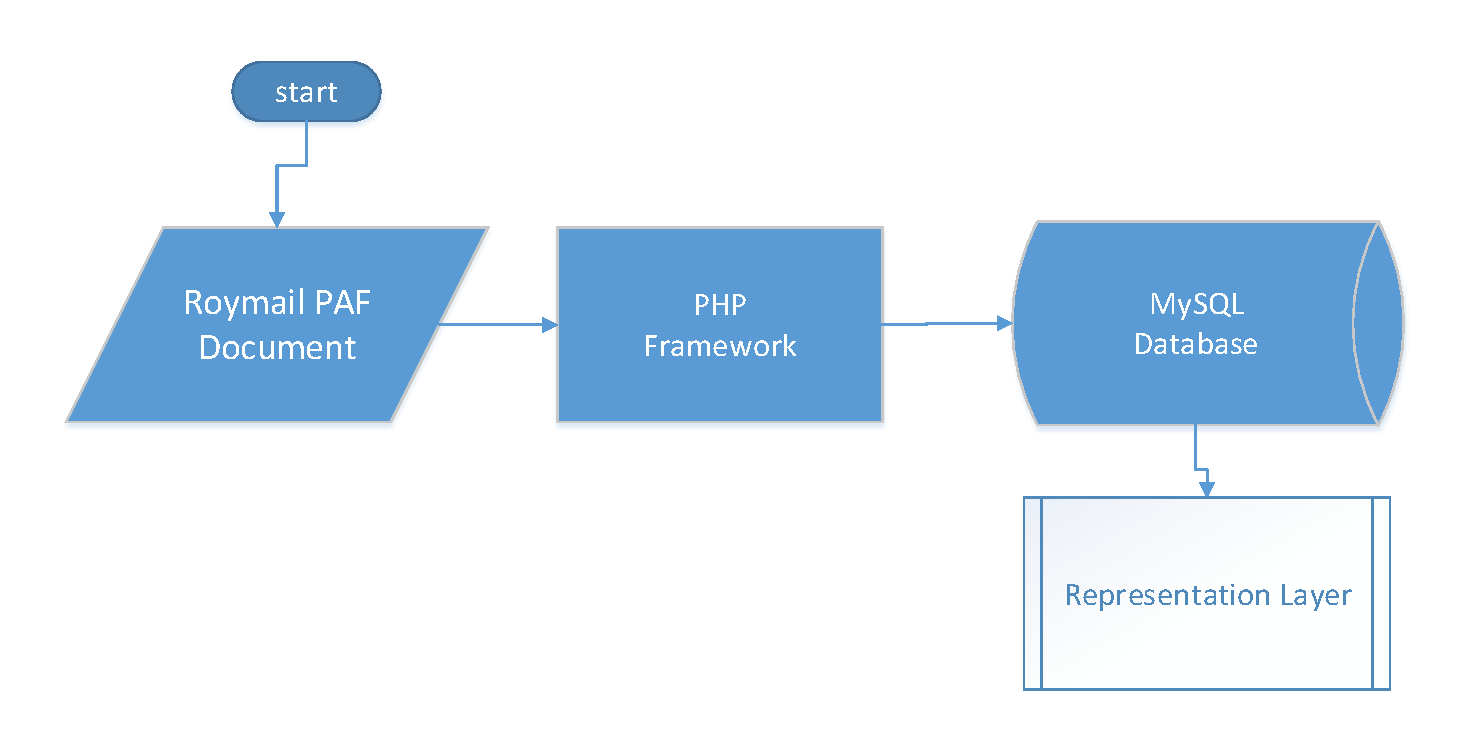
\includegraphics[scale=0.6]{chapter4/data_analysis_exp1}
\caption{Experiment One - UK Geographic Data Set Analysis}
\end{figure}

The Royal Mail PAF data set is quite large which required a special script to convert the file into a MySQL database  to enable future re-use and retrieval. The customised code  removed unwanted and repeated information from the PAF file and normalised the database accordingly for representation purposes in the next step. The refined database consisted of 1.7 million rows which were imported into the MySQL database. The extracted sample code for the raw data conversion into a normalised MySQL format is presented in Listing 1 and Listing 2.

%Python code highlighting
\begin{listing}
\begin{minted}
[
frame=lines,
framesep=2mm,
baselinestretch=1.2,
bgcolor=LightGray,
fontsize=\footnotesize,
linenos
]
{python}

require __DIR__.'/db-config.php';
set_time_limit(3600);
$options = array(
        PDO::MYSQL_ATTR_INIT_COMMAND => 'SET NAMES utf8',
        PDO::ATTR_ERRMODE => PDO::ERRMODE_EXCEPTION,
);
$dbh = new PDO('mysql:dbname='.DB_NAME.';host='.DB_HOST, 
DB_USER, DB_PASS, $options);

$include_columns = array(
        'ORD' => 0,
        'ORC' => 1,
        'SBN' => 2,
        'BNA' => 3,
        'NUM' => 5,
        'DST' => 6,
        'STM' => 7,
        'PTN' => 10,
        'PCD' => 11,
        'CTT' => 14,
        'LGE' => 25,
);

\end{minted}
\caption{PAF Raw Data Set Conversion Sample Code}
\end{listing}

%Python code highlighting
\begin{listing}
\begin{minted}
[
frame=lines,
framesep=2mm,
baselinestretch=1.2,
bgcolor=LightGray,
fontsize=\footnotesize,
linenos
]
{python}

$handle = fopen(__DIR__.'/Luton.csv', 'r');
$row = 0;
$max_rows = 0;
while (($buffer = fgets($handle, 4096)) !== false) {
    $row++;
    $csv_row = str_getcsv($buffer, ',');
    
    $insert_data = array();
    foreach ($include_columns as $col_name => $col_index) {
        $insert_data[strtolower($col_name)] = (string) $csv_row[$col_index];
    }
    
    $sth = $dbh->prepare('INSERT INTO geodata_uk 
    ('.implode(',', array_keys($insert_data)).')
    VALUES('.implode(',', array_fill(0, count($insert_data),
    '?')).')');
    $sth->execute(array_values($insert_data));
    
    if ($max_rows > 0 && $row >= $max_rows) {
        break;
    }
}
fclose($handle);


\end{minted}
\caption{PAF Raw Data Set to MySQL Selected Code 2}
\end{listing}

There were over 150 columns which were reduced to only 9 as depicted in Figure 4.2. This is  important information which  the data representation layer retrieved from the database. The database had rows such as latitude and longitude which were important for location detection while street, county and postcode names were required in the visualised form on an interactive map.


\begin{figure}[H]
\centering
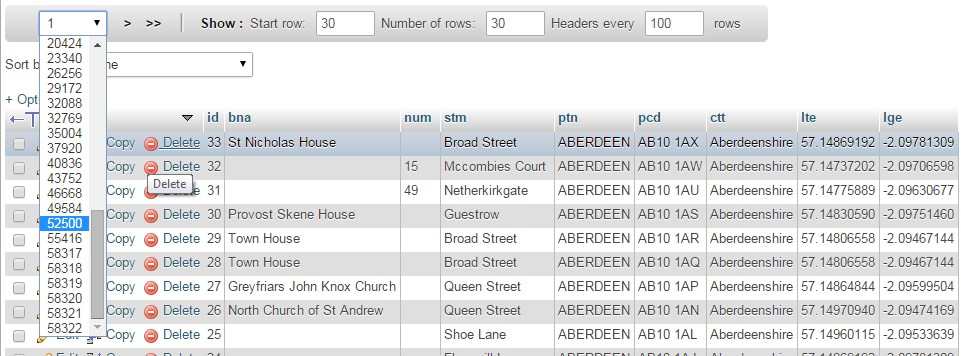
\includegraphics[scale=0.57]{chapter4/experiment_one_database}
\caption{Experiment One - UK Geographic Data Set MySQL}
\end{figure}

The refined information from the MySQL database is then retrieved by additional functions on the interactive map. Information such as latitude and longitude are used for location placement, while postcodes and other information are overlayed on the interactive map.

\subsubsection{Experiment Two - Business Transactional Data}

The business transactional data set and its acquisition is discussed, which is further explained in Chapter 5 in the business transactional experiment. The data set has been taken from a UK based business and covers approximately 7 years of transactional data consisting of around 30 million records of staff information such as logs. Sales operational data has also been imported and utilised in the data analysis and visualisation process. The process of acquiring and analysing data slightly differs from ordinary data sources as the data sets are already optimised and normalised since it is in an enterprise environment. This means the business has existing tools and frameworks which are responsible for data generation and business management and make them available to internal and external applications. Figure 4.3 shows the process of data analysis, where admin or the manager has the ability to pick and choose relevant information for the visualisation process.

\begin{figure}[H]
\centering
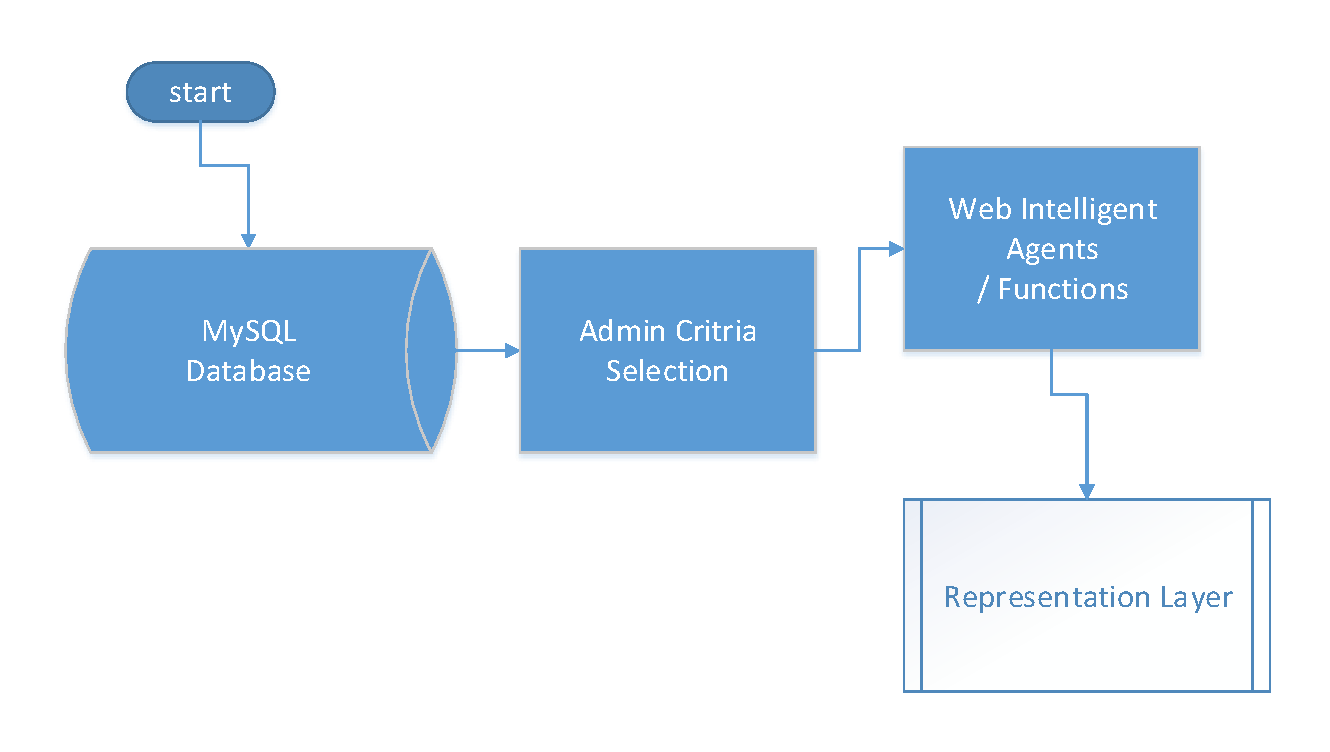
\includegraphics[scale=0.6]{chapter4/data_analysis_exp2a}
\caption{Experiment Two - Business Transactional Data Set in Enterprise Environment}
\end{figure}

Figure 4.4 demonstrates an example database table taken from the MySQL database showing staff members and sales target figures. The admin staff or the manager has options at the interact++ layer to select or deselect a particular staff member through the proposed system - thus the system is directly accessing information through a bespoke interface for the admin and the users. 

\begin{figure}[H]
\centering
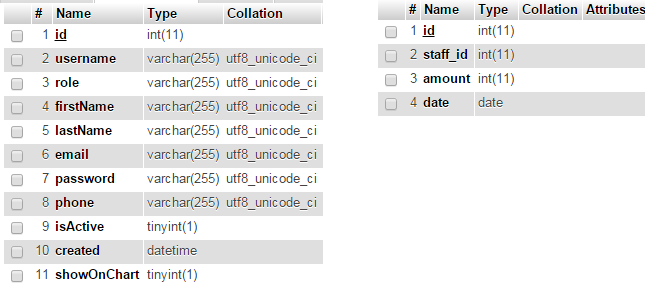
\includegraphics[scale=0.6]{chapter4/exp2_data_analys_db}
\caption{Experiment Two - Business Transactional Data Set Example Tables}
\end{figure}

The user selection and how information is pre-selected or on-demand selected for visualisation is further explained at the interact++ layer. Visualixer is a dedicated tool specially created for individuals and for data sets which are not related to any business application. In other words, data is directly imported into the data analysis model for processing, filtering and mining, which is then pushed into a database for re-use at the representation layer of our visualisation model through bespoke web intelligent agents.


\begin{figure}[H]
\centering
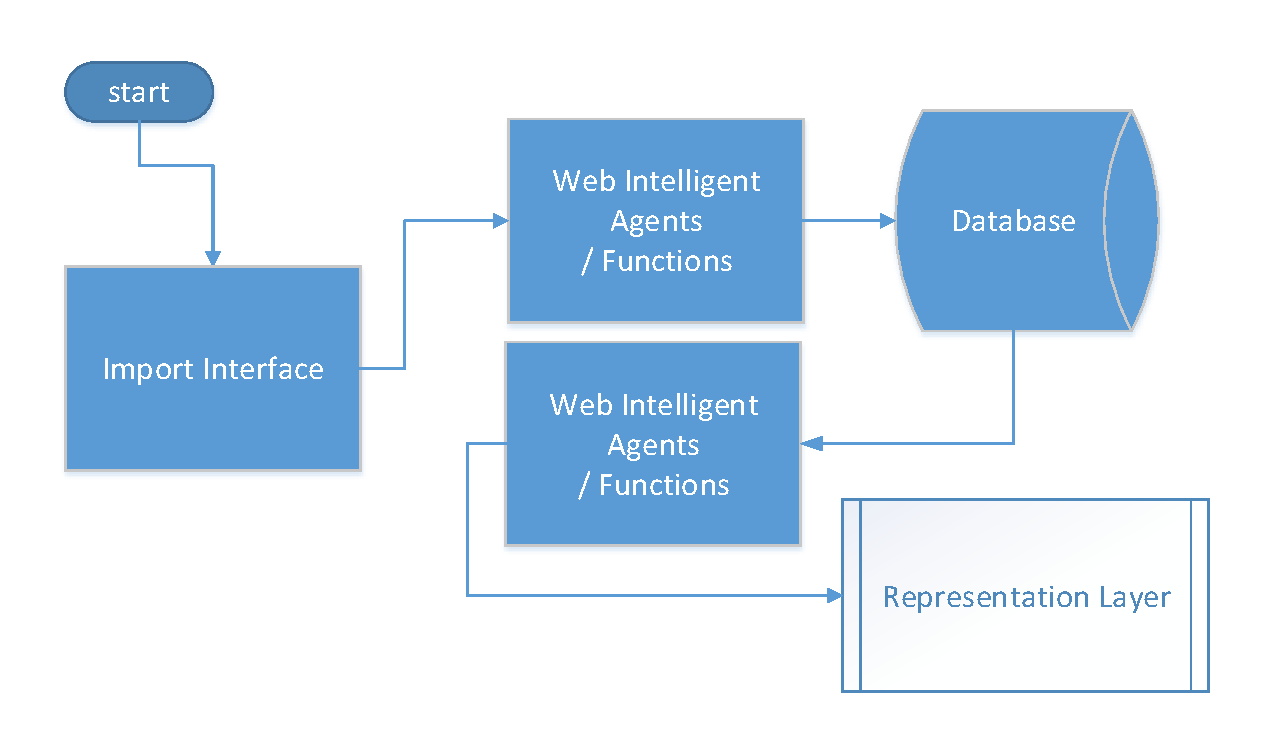
\includegraphics[scale=0.7]{chapter4/data_analysis_exp2b}
\caption{Experiment Two - Data Analysis Process in Visualixer}
\end{figure}

As shown in Figure 4.5, the data is first imported by the user through an interface layer and it goes into the data analysis model.  Where it is refined, unwanted information is removed and normalised and clean data is passed onto the MySQL database where it can be retrieved by the system functions at a later stage for visualisation. A sample import code has been shown in Listing 3, however the tool is created in a PHP framework which comes with thousands of lines of code and it is not possible to demonstrate the full system code. Instead, system features are demonstrated.

%Python code highlighting
\begin{listing}[ht]
\begin{minted}
[
frame=lines,
framesep=2mm,
baselinestretch=1.2,
bgcolor=LightGray,
fontsize=\footnotesize,
linenos
]
{python}
  .....
        public function upload()
        { 
            $this->load->model('import_model');
            $this->load->helper('file');
            $user_data = $this->session->userdata('id');
           
            //$path = './upload/'.$user_data;
            $path = './upload/temp';
            if(!is_dir($path)) //create the folder if it's not already exists
            {
              mkdir($path,0777,TRUE);
            } 
            $this->load->helper('form');
            $config['upload_path'] = $path;
            $config['allowed_types'] = '*';
            $config['max_size']	= '';
            ......



\end{minted}
\caption{Experiment Two - Visualixer Import Function Highlights }
\end{listing}

\subsection{Data Representation}

In this section, a brief discussion on the representation of the data which has been analysed by acquisition and data analysis layer in the previous step is shown. Firstly, in  Experiment One, a data set will be discussed which has been adapted from the Royal Mail PAF address which has been refined in the data analysis step; data required for this experiment has already been normalised and is available in the MySQL format for the web intelligent agents (PHP functions) to be retrieved for the representation layer, as illustrated in Figure 4.6.

\begin{figure}[H]
\centering
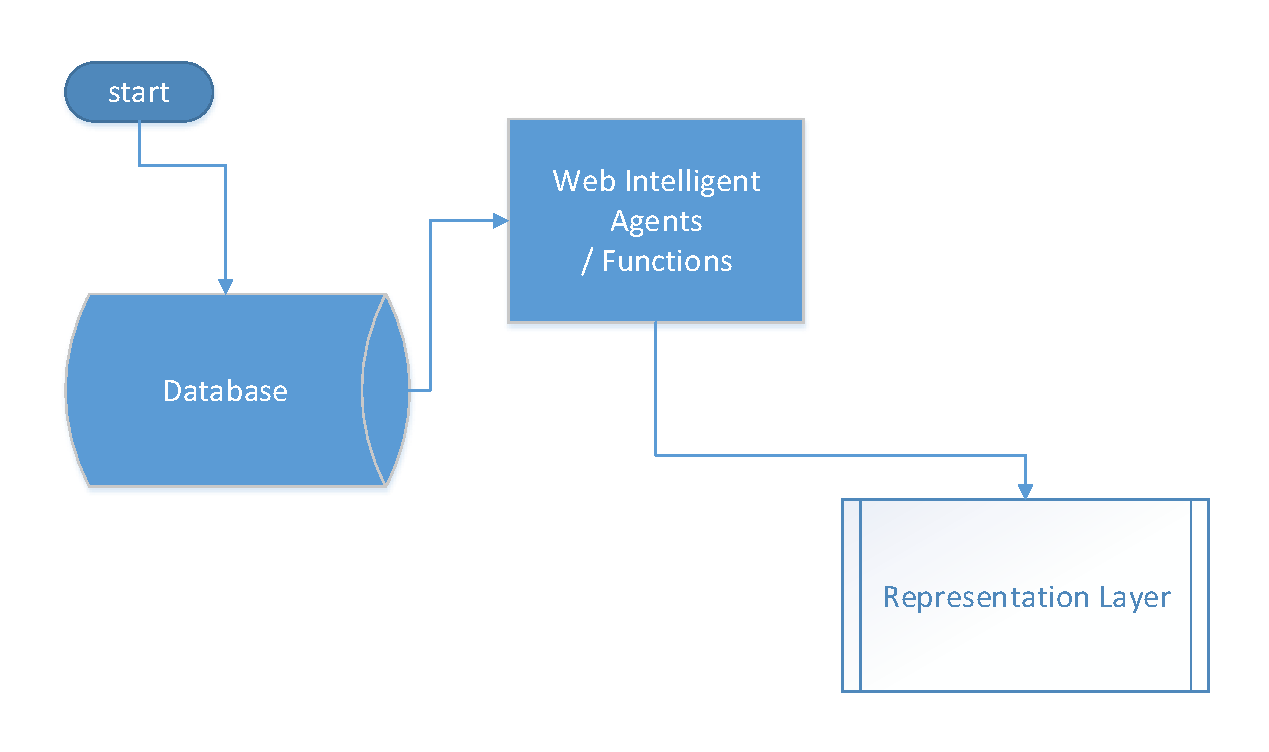
\includegraphics[scale=0.6]{chapter4/respresentation_exp1}
\caption{Experiment One - Data Representation Process}
\end{figure}

The data retrieved from the database has been represented with an interactive map. The data mashup aspects of the visualisation model are introduced and processed at this layer. Mashup tools are convenient to program and develop quick and short applications which support other processing and analysis functions within the proposed system. A short interactive map initialisation code shows the process in Listing 4.

\begin{listing}[ht]
\begin{minted}
[
frame=lines,
framesep=2mm,
baselinestretch=1.2,
bgcolor=LightGray,
fontsize=\footnotesize,
linenos
]
{python}
  .....
  function initializeMap() {
  map = new google.maps.Map($('#map-canvas')[0], mapOptions);
  map.controls[google.maps.ControlPosition.TOP_LEFT].push($('#topbar')[0]);

  /* attach searches */
  $('#address').autocomplete({
    source: mapAreas,
    select: function(event, ui) {
      var areaName = ui.item.value.toUpperCase();
      var matchLen = 0;
      var matchArea;
      for(var areaKey in mapAreaBounds) {
        if (name.length == 1 && areaKey == areaName) {
          matchArea = areaKey;
          matchLen = 1;

          break;
        } else {
          var pos = areaKey.indexOf(areaName);
          var len = areaKey.length;
          if (pos == 0) {
            if (matchLen == 0 || len > matchLen) {
              matchArea = areaKey;
              matchLen = len;
            }
          }
        }
      }

            ......



\end{minted}
\caption{Experiment One - Interactive Map Initialisation Example Code }
\end{listing}

The data representation process is explained at the enterprise level or in applications where data is already normalised and in a known state. The data is retrieved from the database through web intelligent agents (PHP functions) and then made available to users at the interact++ layer; the user has the ability to pick and choose what information users may want to visualise and the information is then pushed into the database again for future re-use purposes. Web intelligent agents then remember user choice or preferences and push specified data into the representation layer, which then generates visualised information for the user at the interact++ layer; the flow chart of the process is manifested in Figure 4.7.

\begin{figure}[H]
\centering
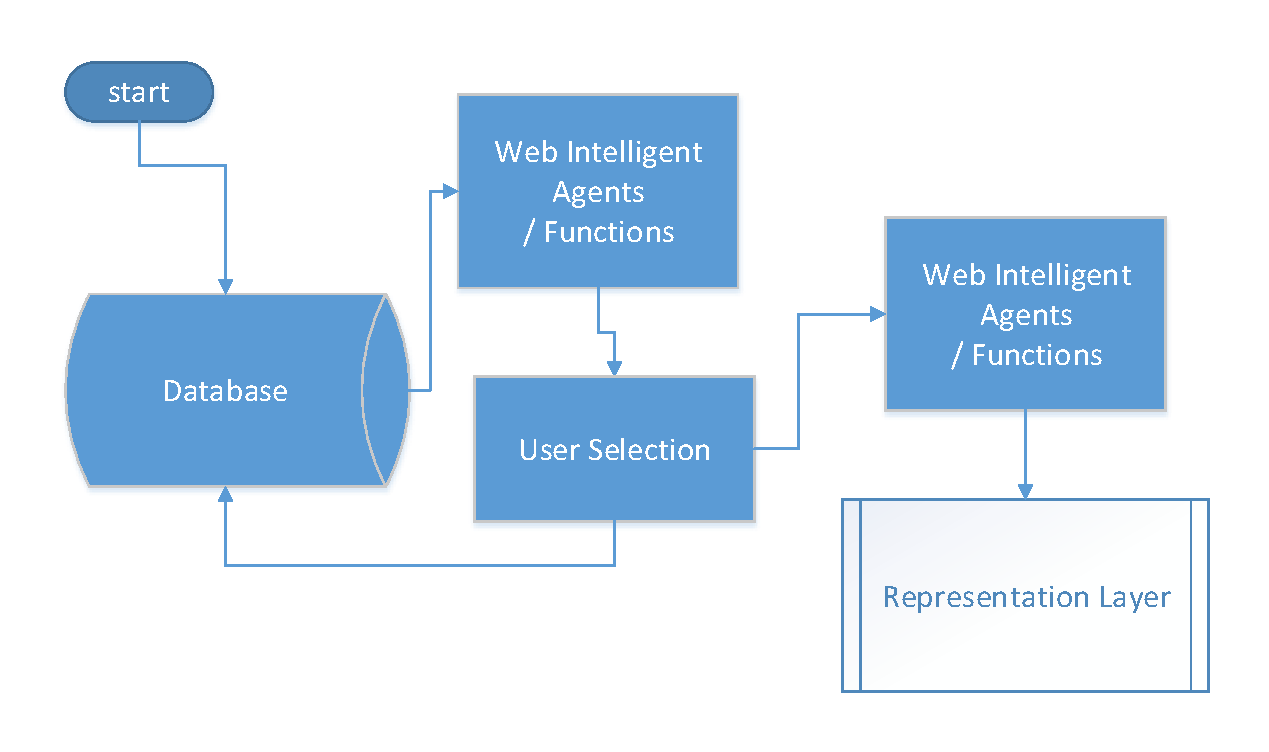
\includegraphics[scale=0.6]{chapter4/data_representation_exp2a}
\caption{Experiment One - Visualisation Model from Various Perspective}
\end{figure}

The code sample in Listing 5 shows the basic functions for data representation at this layer. The demonstrated code is only an example and an extracted partial code of how this process works and how data is retrieved from the database for  representation purposes.


\begin{listing}[ht]
\begin{minted}
[
frame=lines,
framesep=2mm,
baselinestretch=1.2,
bgcolor=LightGray,
fontsize=\footnotesize,
linenos
]
{python}
  .....
use Symfony\Bundle\FrameworkBundle\Controller\Controller;
use Symfony\Component\HttpFoundation\Request;
use Symfony\Component\HttpFoundation\ResponseHeaderBag;
use Sensio\Bundle\FrameworkExtraBundle\Configuration\Route;
use Premier\CoachhireBundle\Form\Type\Quote\ListFilterType;
use Premier\CoachhireBundle\Entity\Quote;
use Premier\CoachhireBundle\Entity\Invoice;
use Doctrine\ORM\Query;
use DateTime;
use PDO;

    public function latestSalesStatsAction(Request $request)
    {
        $em = $this->getDoctrine()->getEntityManager();

        $months = range(1, 12);
        $years = range(date('Y')-2, date('Y'));
        $defaultData = array('month' => date('n'), 'year' => date('Y'));

        $form = $this->createFormBuilder($defaultData)
            ->add('month', 'choice', 
            array('choices' => 
            array_combine($months, $months), 'required' => false))
	        ->add('year', 'choice', array(
	        'choices' => array_combine($years, $years), 
	        'required' => false))
	        ->getForm()
    	;

        $stats = array(
            'enquiry'   => array(0, 0),
            'processing'   => array(0, 0),
            'booked'    => array(0, 0),
            'declined'  => array(0, 0),
            'following' => array(0, 0),
            'processing_active' => array(0, 0),
            'total_active'   => array(0, 0),
        );
        ......



\end{minted}
\caption{Experiment Two - Data Representation Preparation Example Code }
\end{listing}
\clearpage

In a non-enterprise environment where data is not in SQL format, the Visualixer converts data into MySQL in the previous section (Acquisition and Data Analysis). The Visualixer at the interact++ layer gives the user the choice to select information for visualisation. The user retrieves information from the database through web intelligent agents (PHP functions) and once the information is retrieved, the user then submits the information into the representation model where the information is visualised, as shown in Figure 4.8.

\begin{figure}[H]
\centering
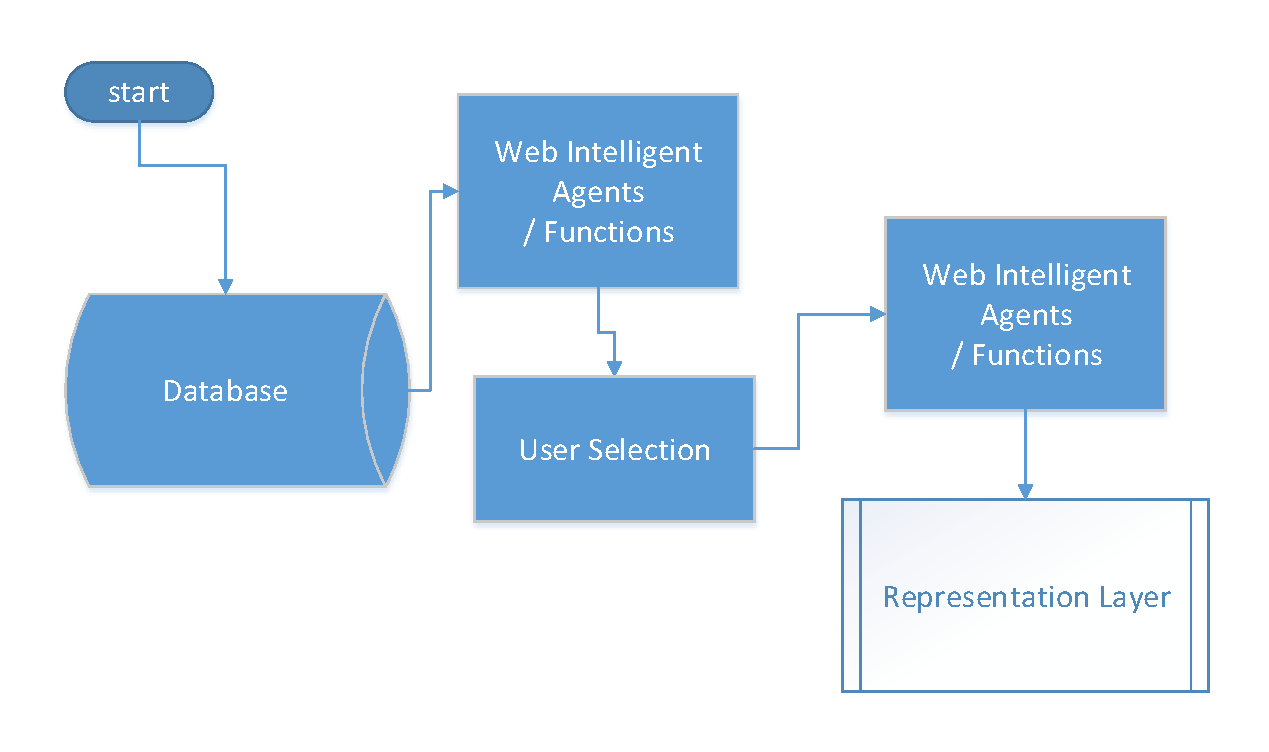
\includegraphics[scale=0.6]{chapter4/data_representation_exp2b}
\caption{Experiment Two - Data Representation in Visualixer}
\end{figure}

The data representation of different data sets is explained with various flow charts and with brief code examples. In the next section the interact++ layer will be discussed, showing how users interact with the system. 

\subsection{User Interaction}

User interaction is an important aspect of any application. User interaction relates to all elements depending how users react to an application and how applications react to the user responses \cite{hix1993developing}. The interactive layer is mostly designed and developed using front end technologies such as HTML and CSS with the help of JQuery and other supporting tools. A variety of mashup applications are also utilised in the development process. Bootstrap is also used in the creation of user interfaces. The system adaptability and user experience has been enhanced with JQuery and Javascript functions and applications by giving auto-complete options to users. In Experiment One - with UK geographic data - AJAX (mostly JAVA functions) is used for better interface, user and application interaction. However, more conventional technologies such as HTML5 and CSS3 are used in Visualixer (the tool which is developed for non-enterprise data sets). In Experiment Two - with business transactional data - a more enhanced user interface is provided as most of the system is controlled by the users to issue instruction to the application for both data analysis and data representation. 

\subsection{Exporting Reports}

Data export features of the system are discussed. Generating and analysing data and information is a very useful process, however information not stored for future use does not add much value to the application. The export feature of reports and data is a vital part of the visualisation model. Therefore this has been precisely considered and developed to equip system users to export and save data for external use. Experiment One -  with the UK geographic data, the user has the option to export visualised maps into various formats such as JPEG, GIF, PNG, PDFs. The exported files are of high resolution and quality print. Experiment Two - with an enterprise environment, this also gives the ability to end users to export charts and graphs into JPEG, GIF, PNG and PDFs. The system also gives the user an option to extract utilised data in CSVs and they are accessible through APIs for external applications. These export features are powered by customised and bespoke functions and partial mashup applications are also used in the system development. Using Visualixer in Experiment Two also gives the same ability to the users to export generated charts and graphs in various formats. 

\section{Design and Development Overview of Experiment One}

A brief overview of Experiment One is presented in Figures 4.9 and 4.10, showing the visualisation model, development process and technologies, and from the end user perspective. 

\begin{figure}
\centering
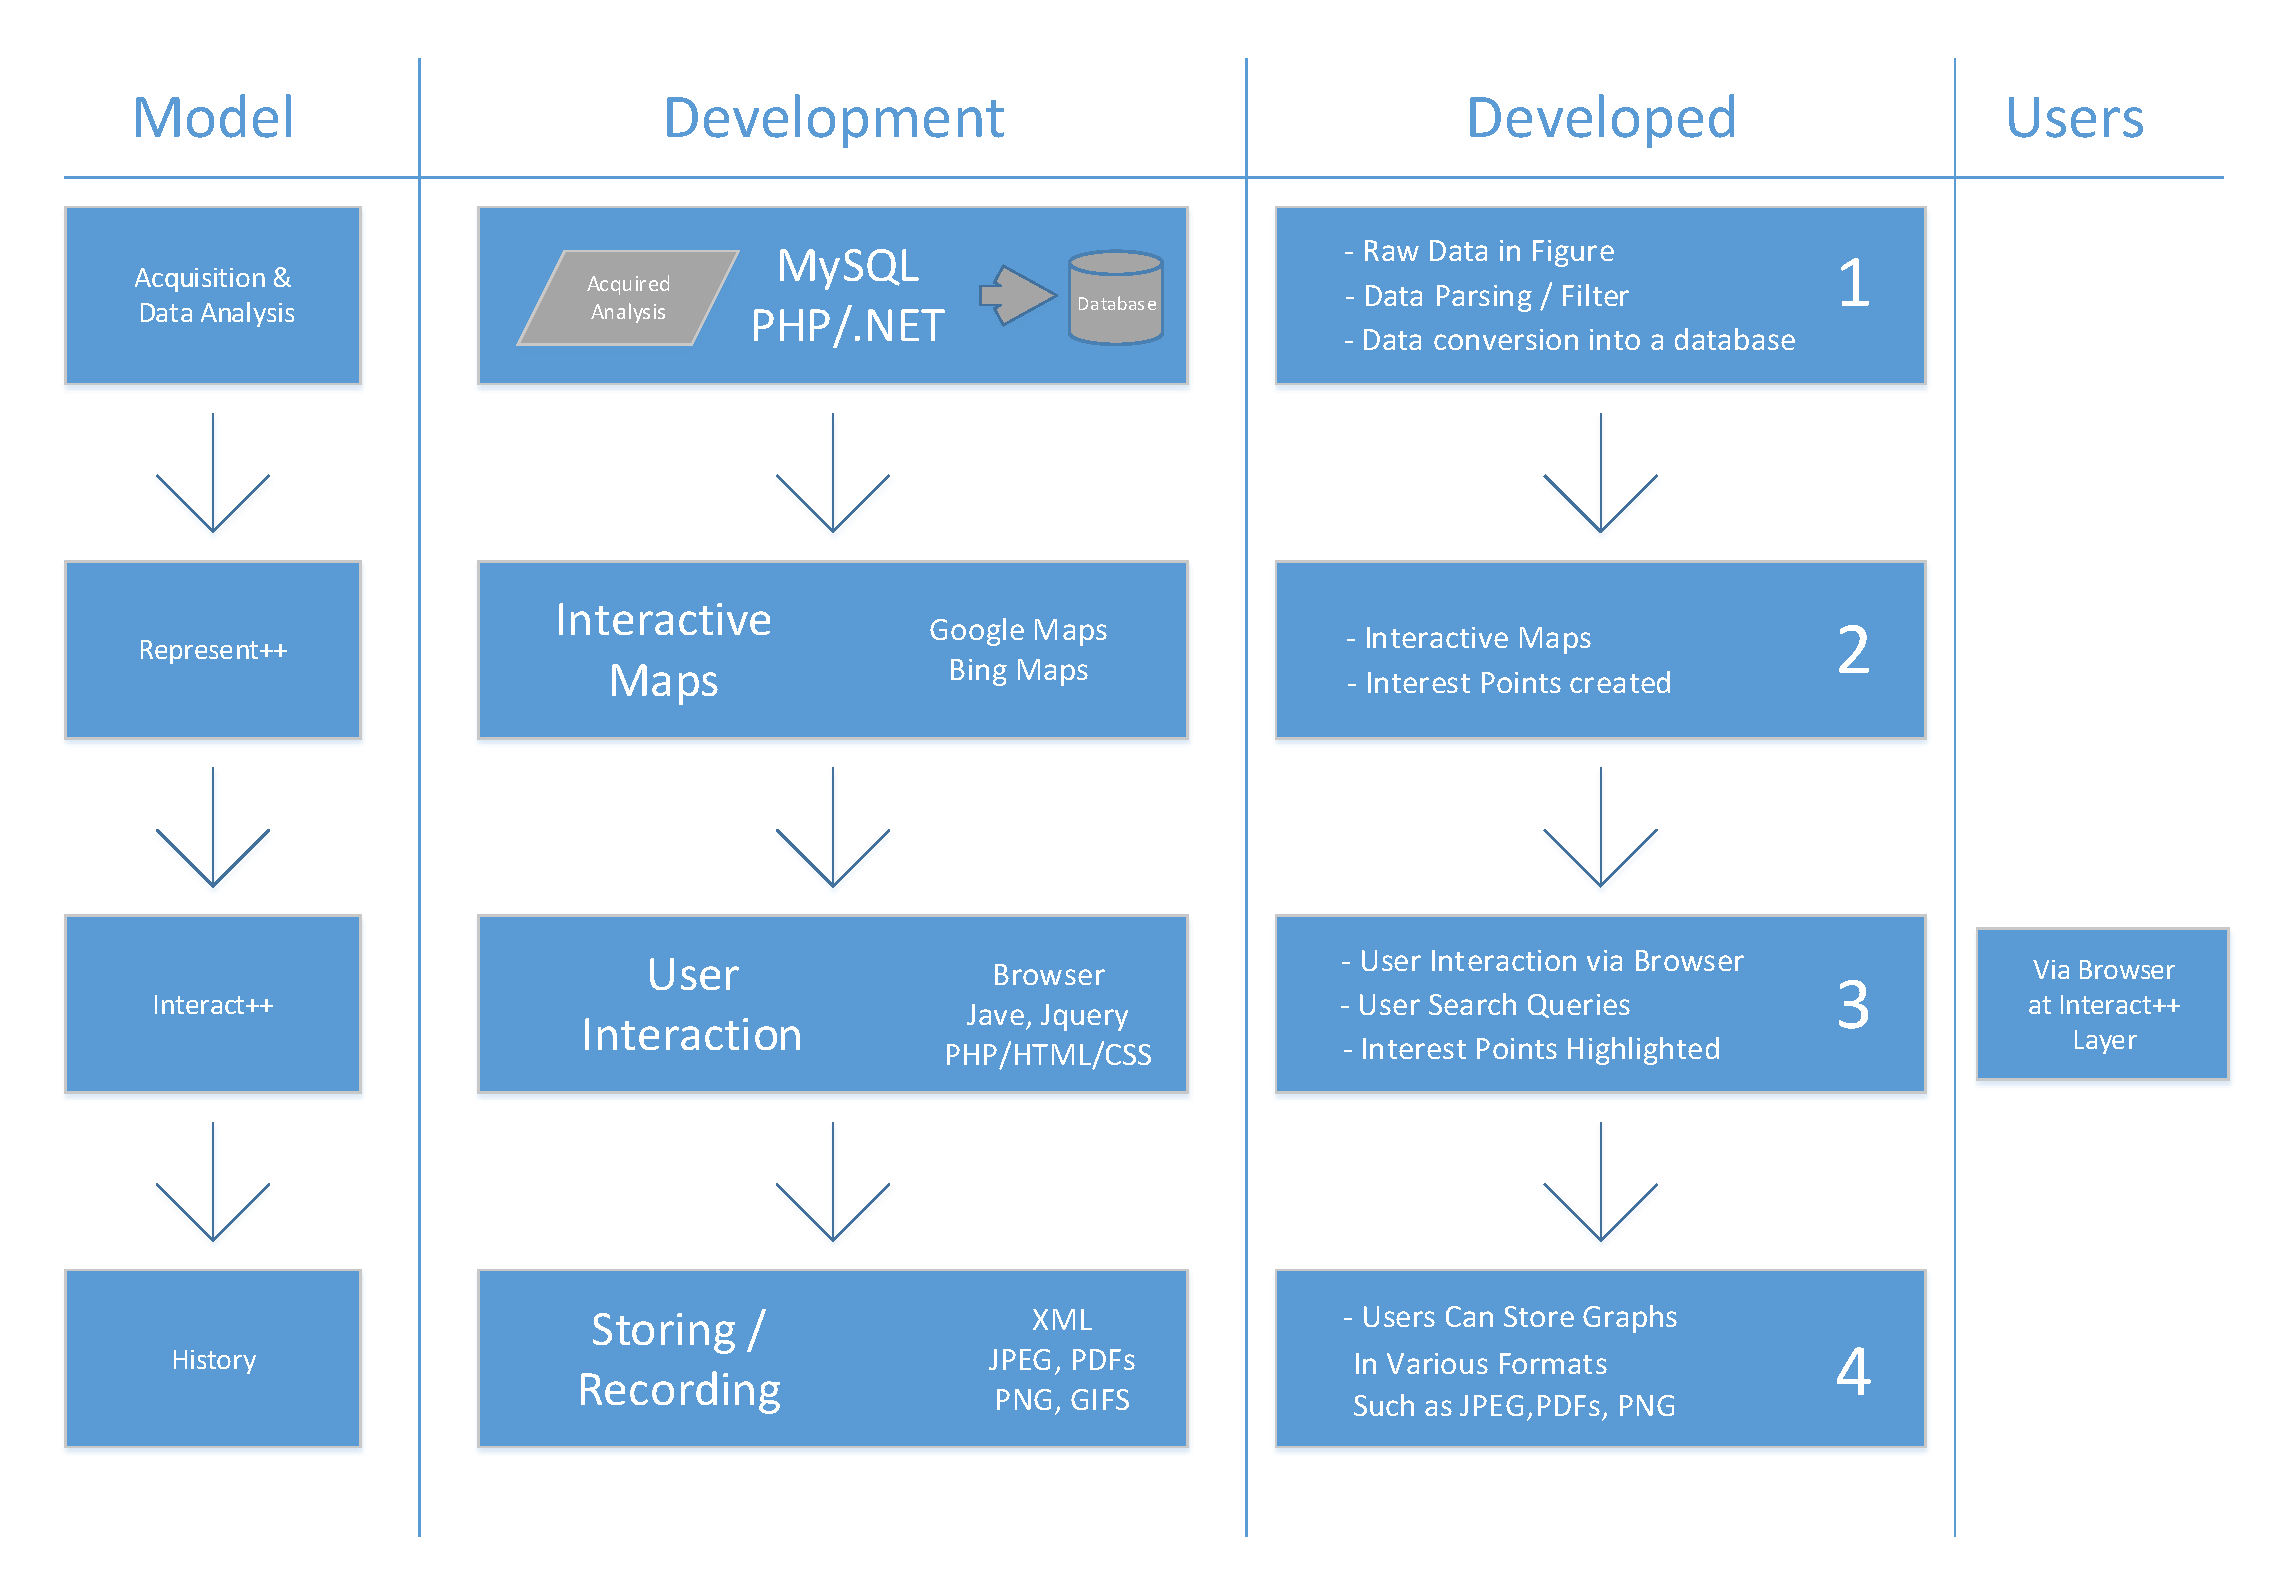
\includegraphics[scale=0.37]{chapter4/system_full_overview}
\caption{Experiment One - System Overview}
\end{figure}

\begin{figure}
\centering
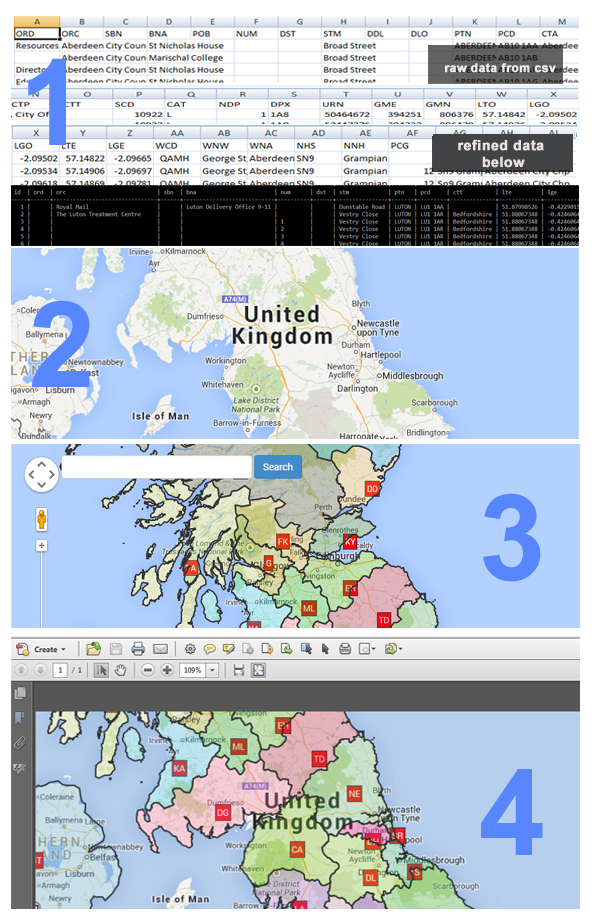
\includegraphics[scale=0.7]{chapter4/actual_overview}
\caption{Experiment One - Actual System Overview}
\end{figure}

In Figure 4.10, actual screen shots are taken from the application. The numbers 1-4 on the screen shots refer to layers in the information visualisation model. The process is started from the acquisition and data analysis point. Data is visualised at the represent++ layer. User interaction takes place at the interact++ layer, while export options are available at the history layer. 

\section{Design and Development Overview of Experiment Two}

A brief overview of Experiment Two is discussed in this section. Experiment Two in Chapter 5 is further divided into two parts. The first part of the experiment deals with data sets which are already in a well developed application and data sets are either directly accessed from the MySQL database or through APIs and web services. The model design shows the main four stages, starting from acquisition and data analysis, data representation, user interaction and exporting of generated reports. The development process is also defined and instructions are given to define what kind of technologies could be used in order to replicate or utilise the same visualisation process and model. Developed application and its user levels with different privileges are also explained in the overview chart in Figure 4.11.

\begin{figure}
\centering
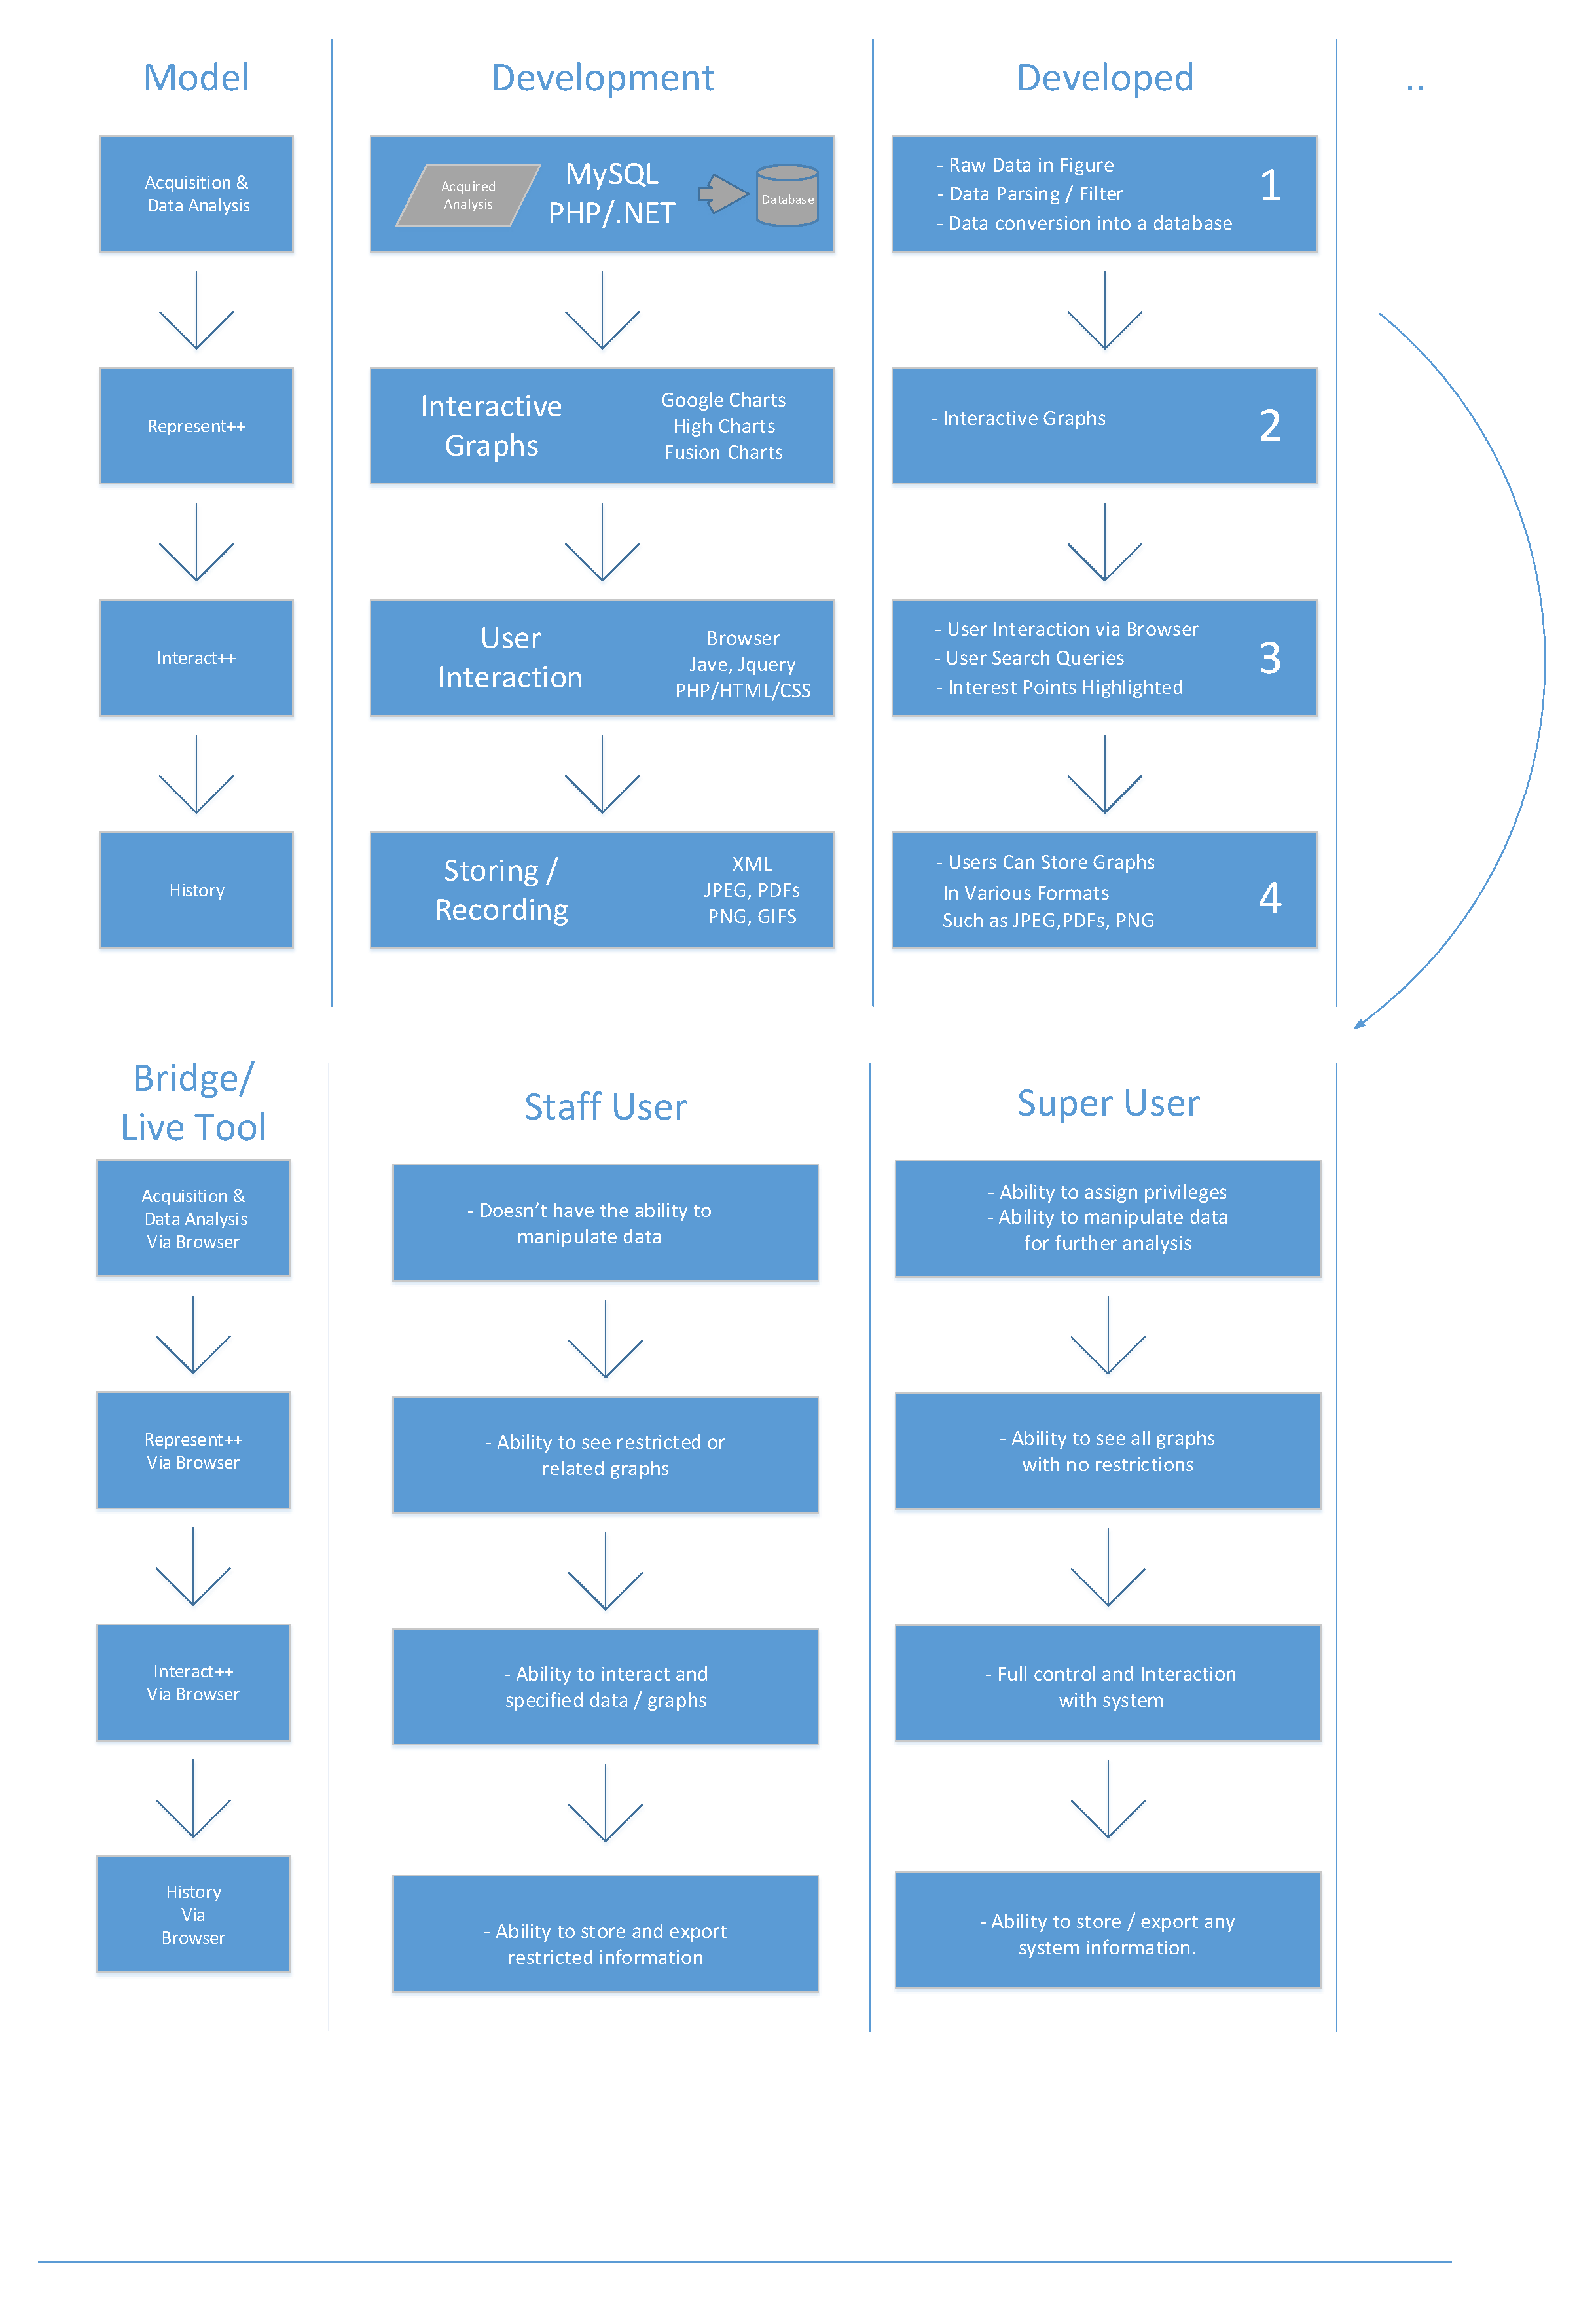
\includegraphics[scale=0.37]{chapter4/overview_ex2a}
\caption{Experiment Two  - System Overview}
\end{figure}

Figure 4.12 illustrates actual screen shots, starting from MySQL databases, showing how users see the information at the front end and then the data representation and interaction with the user in Step 3. Step 4 shows options to export information such as graphs and structural data into various formats. The same area of the figure also shows other relevant sections of data visualisation including multi-coordinate visualisation and multiple attribute data visualisation made available to users at the interface layer.

\begin{figure}
\centering
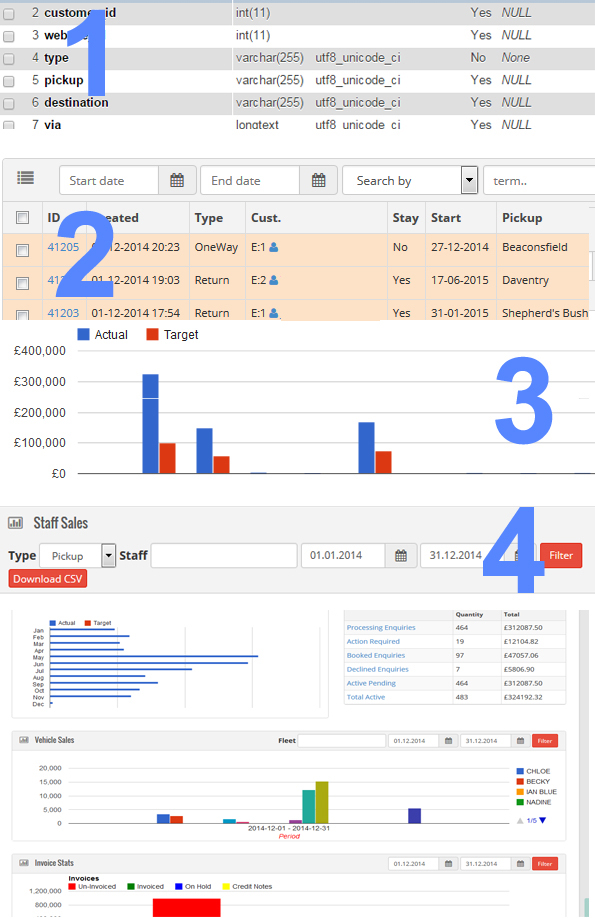
\includegraphics[scale=0.7]{chapter4/exp2a}
\caption{Experiment Two  - Enterprise 2.0 Application Screen shots}
\end{figure}


In the process for data sets which are in a non-enterprise format or not in normalised form, the data sets are imported into the acquisition and analysis layer for refinement and analysis for data representation at a later layer. Figure 4.11 demonstrates various steps from the initial theoretical model to the development process and in-development phases, showing different type of user access. The information visualisation model layers are highlighted in the first column while development scenarios explained in the second column. Developed aspects of the visualisation model are highlighted in the third column. Bridge refers to Enterprise 2.0 environment where web intelligent agents are configured to retrieve information from the data set in a real time environment. Live tool refers to Visualixer which is a dedicated tool based on the four layers of proposed visualisation model. Various aspects of users highlighted in the last two columns of the flowchart. Figure 4.13 manifests screen shots from the live system (Visualixer). The first step deals with raw data and converts it into normalised and database format; the web intelligent agents (PHP functions) read information from the database allowing users to select the required fields for visualisation and then pass them on to the data representation layer for visualisation. The user's interaction is achieved at the interact++ layer with the help of HTML5, CSS3, AJAX and JQuery technologies for clean and easy to use interfaces.

\begin{figure}[H]
\centering
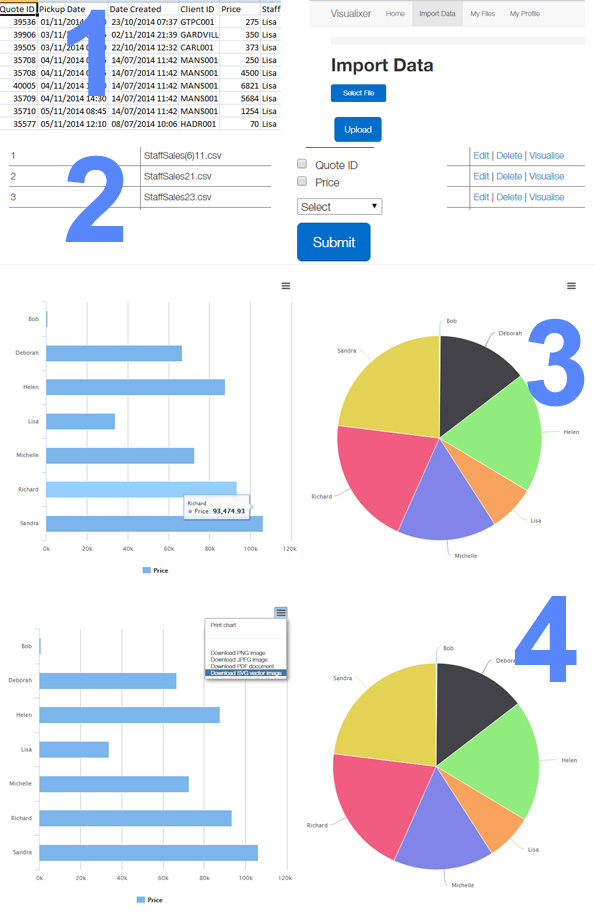
\includegraphics[scale=0.7]{chapter4/exp2b}
\caption{Experiment Two B  - Visualixer Tool Screen shots}
\end{figure}

\section{Summary}

The visualisation model has been revisited from Chapter 3 with abstract proposed system flow charts presented from the overall model and each layer of the model. The data processing and visualisation along with user interaction and data export are explained with a system flowchart and the technologies used in the mechanism.

In the second part of the chapter, each layer of the visualisation model has been explained with an example code from the actual applications developed for the experiments accompanied by flowcharts for each step. An overview of the two experiments in Chapters 5 and 6 are briefly discussed with screen shots from the application. The system process is examined at each individual layer of the information visualisation model. 

The objective of this chapter was to give a better understanding to the reader of how the model has been adapted and developed. The two experiments are demonstrated with screen shots for a brief overview of the system structure and design. The next chapter shows detailed information about the data set used in the experiment and how data is visualised by the system covering all four layers of the visualisation model proposed in this research.
